\begin{minipage}{.6\linewidth}
	\vspace{-1cm}
	\item O homem senta na cadeira giratória segurando dois pesos de \SI{2.5}{\kilogram} com seus braços estendidos. Se ele está girando a \SI{3}{\radian/\second} nessa posição, determine sua velocidade angular quando os pesos são aproximados e seguros a \SI{.09}{\meter} do eixo de rotação. Suponha que ele tem uma massa de \SI{80}{\kilogram} e um raio de giração $k_{z}=\SI{.165}{\meter}$ em relação ao eixo $z$. Despreze a
	massa de seus braços e a dimensão dos pesos para o cálculo.\\
	
	\import{../answers}{answer-9}
\end{minipage}
\begin{minipage}{.4\linewidth}
	\begin{flushright}
		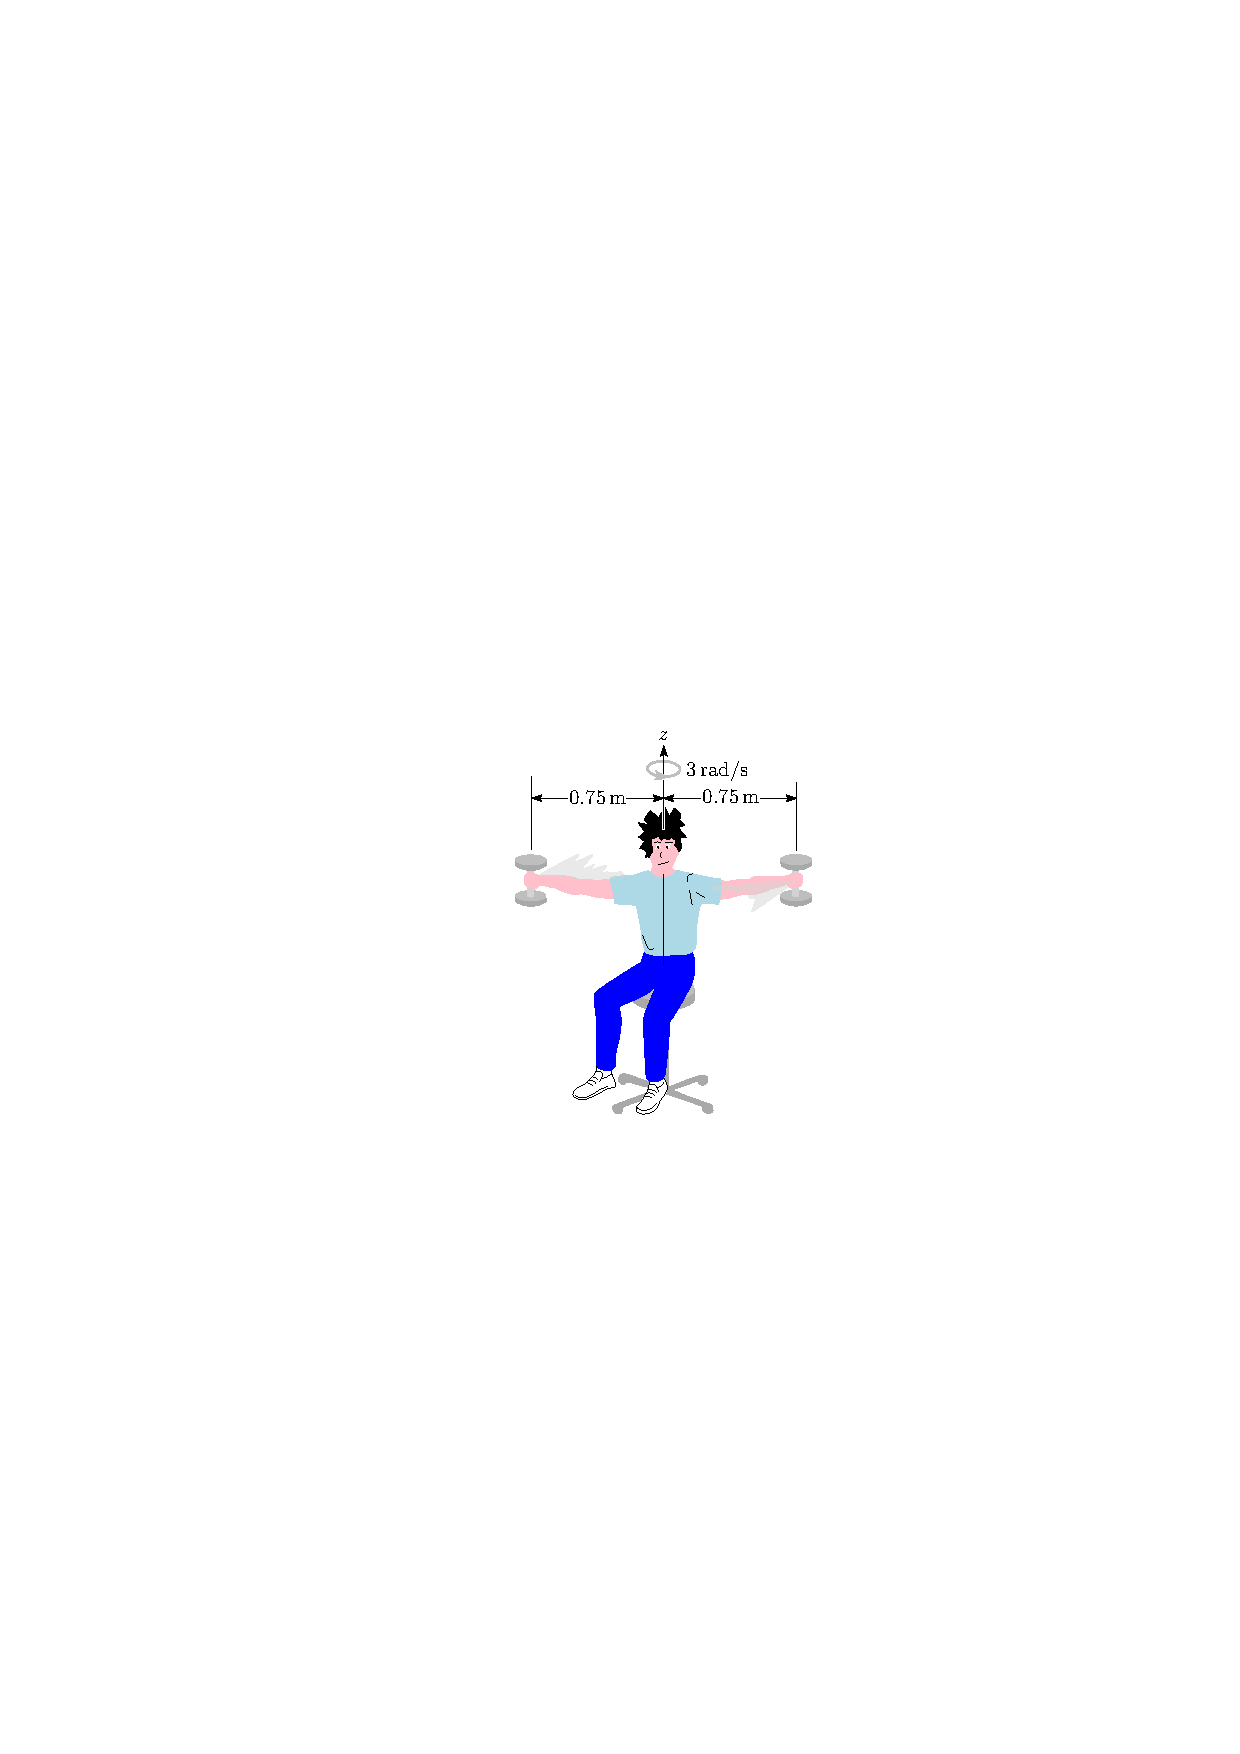
\includegraphics[scale=1.2]{../../images/draw_6}
	\end{flushright}

\end{minipage}